\documentclass[12pt,a4paper]{article}
	%[fleqn] %%% --to make all equation left-algned--

% \usepackage[utf8]{inputenc}
% \DeclareUnicodeCharacter{1D12A}{\doublesharp}
% \DeclareUnicodeCharacter{2693}{\anchor}
% \usepackage{dingbat}
% \DeclareRobustCommand\dash\unskip\nobreak\thinspace{\textemdash\allowbreak\thinspace\ignorespaces}
\usepackage[top=2in, bottom=1in, left=1in, right=1in]{geometry}
%\usepackage{fullpage}

\usepackage{fancyhdr}\pagestyle{fancy}\rhead{Stephanie Wang}\lhead{EE236B homework 7}

\usepackage{amsmath,amssymb,amsthm,amsfonts,microtype,stmaryrd}
	%{mathtools,wasysym,yhmath}

\usepackage[usenames,dvipsnames]{xcolor}
\newcommand{\blue}[1]{\textcolor{blue}{#1}}
\newcommand{\red}[1]{\textcolor{red}{#1}}
\newcommand{\gray}[1]{\textcolor{gray}{#1}}
\newcommand{\fgreen}[1]{\textcolor{ForestGreen}{#1}}

\usepackage{mdframed}
	%\newtheorem{mdexample}{Example}
	\definecolor{warmgreen}{rgb}{0.8,0.9,0.85}
	% --Example:
	% \begin{center}
	% \begin{minipage}{0.7\textwidth}
	% \begin{mdframed}[backgroundcolor=warmgreen, 
	% skipabove=4pt,skipbelow=4pt,hidealllines=true, 
	% topline=false,leftline=false,middlelinewidth=10pt, 
	% roundcorner=10pt] 
	%%%% --CONTENTS-- %%%%
	% \end{mdframed}\end{minipage}\end{center}	

\usepackage{graphicx} \graphicspath{{}}
	% --Example:
	% \includegraphics[scale=0.5]{picture name}
%\usepackage{caption} %%% --some awful package to make caption...

\usepackage{hyperref}\hypersetup{linktocpage,colorlinks}\hypersetup{citecolor=black,filecolor=black,linkcolor=black,urlcolor=blue,breaklinks=true}

%%% --Text Fonts
%\usepackage{times} %%% --Times New Roman for LaTeX
%\usepackage{fontspec}\setmainfont{Times New Roman} %%% --Times New Roman; XeLaTeX only

%%% --Math Fonts
\renewcommand{\v}[1]{\ifmmode\mathbf{#1}\fi}
%\renewcommand{\mbf}[1]{\mathbf{#1}} %%% --vector
%\newcommand{\ca}[1]{\mathcal{#1}} %%% --"bigO"
%\newcommand{\bb}[1]{\mathbb{#1}} %%% --"Natural, Real numbers"
%\newcommand{\rom}[1]{\romannumeral{#1}} %%% --Roman numbers

%%% --Quick Arrows
\newcommand{\ra}[1]{\ifnum #1=1\rightarrow\fi\ifnum #1=2\Rightarrow\fi\ifnum #1=3\Rrightarrow\fi\ifnum #1=4\rightrightarrows\fi\ifnum #1=5\rightleftarrows\fi\ifnum #1=6\mapsto\fi\ifnum #1=7\iffalse\fi\fi\ifnum #1=8\twoheadrightarrow\fi\ifnum #1=9\rightharpoonup\fi\ifnum #1=0\rightharpoondown\fi}

%\newcommand{\la}[1]{\ifnum #1=1\leftarrow\fi\ifnum #1=2\Leftarrow\fi\ifnum #1=3\Lleftarrow\fi\ifnum #1=4\leftleftarrows\fi\ifnum #1=5\rightleftarrows\fi\ifnum #1=6\mapsfrom\ifnum #1=7\iffalse\fi\fi\ifnum #1=8\twoheadleftarrow\fi\ifnum #1=9\leftharpoonup\fi\ifnum #1=0\leftharpoondown\fi}

%\newcommand{\ua}[1]{\ifnum #1=1\uparrow\fi\ifnum #1=2\Uparrow\fi}
%\newcommand{\da}[1]{\ifnum #1=1\downarrow\fi\ifnum #1=2\Downarrow\fi}

%%% --Special Editor Config
\renewcommand{\ni}{\noindent}
\newcommand{\onum}[1]{\raisebox{.5pt}{\textcircled{\raisebox{-1pt} {#1}}}}

\newcommand{\claim}[1]{\underline{``{#1}":}}

\renewcommand{\l}{\left}\renewcommand{\r}{\right}

\newcommand{\casebrak}[4]{\left \{ \begin{array}{ll} {#1},&{#2}\\{#3},&{#4} \end{array} \right.}
%\newcommand{\ttm}[4]{\l[\begin{array}{cc}{#1}&{#2}\\{#3}&{#4}\end{array}\r]} %two-by-two-matrix
%\newcommand{\tv}[2]{\l[\begin{array}{c}{#1}\\{#2}\end{array}\r]}

\def\dps{\displaystyle}

\let\italiccorrection=\/
\def\/{\ifmmode\expandafter\frac\else\italiccorrection\fi}


%%% --General Math Symbols
\def\bc{\because}
\def\tf{\therefore}

%%% --Frequently used OPERATORS shorthand
\newcommand{\INT}[2]{\int_{#1}^{#2}}
% \newcommand{\UPINT}{\bar\int}
% \newcommand{\UPINTRd}{\overline{\int_{\bb R ^d}}}
\newcommand{\SUM}[2]{\sum\limits_{#1}^{#2}}
\newcommand{\PROD}[2]{\prod\limits_{#1}^{#2}}
\newcommand{\CUP}[2]{\bigcup\limits_{#1}^{#2}}
\newcommand{\CAP}[2]{\bigcap\limits_{#1}^{#2}}
% \newcommand{\SUP}[1]{\sup\limits_{#1}}
% \newcommand{\INF}[1]{\inf\limits_{#1}}
\DeclareMathOperator*{\argmin}{arg\,min}
\DeclareMathOperator*{\argmax}{arg\,max}
\newcommand{\pd}[2]{\frac{\partial{#1}}{\partial{#2}}}
\def\tr{\text{tr}}

\renewcommand{\o}{\circ}
\newcommand{\x}{\times}
\newcommand{\ox}{\otimes}

\newcommand\ie{{\it i.e. }}
\newcommand\wrt{{w.r.t. }}
\newcommand\dom{\mathbf{dom\:}}

%%% --Frequently used VARIABLES shorthand
\def\R{\ifmmode\mathbb R\fi}
\def\N{\ifmmode\mathbb N\fi}
\renewcommand{\O}{\mathcal{O}}

\newcommand{\dt}{\Delta t}
\def\vA{\mathbf{A}}
\def\vB{\mathbf{B}}\def\cB{\mathcal{B}}
\def\vC{\mathbf{C}}
\def\vD{\mathbf{D}}
\def\vE{\mathbf{E}}
\def\vF{\mathbf{F}}\def\tvF{\tilde{\mathbf{F}}}
\def\vG{\mathbf{G}}
\def\vH{\mathbf{H}}
\def\vI{\mathbf{I}}\def\cI{\mathcal{I}}
\def\vJ{\mathbf{J}}
\def\vK{\mathbf{K}}
\def\vL{\mathbf{L}}\def\cL{\mathcal{L}}
\def\vM{\mathbf{M}}
\def\vN{\mathbf{N}}\def\cN{\mathcal{N}}
\def\vO{\mathbf{O}}
\def\vP{\mathbf{P}}
\def\vQ{\mathbf{Q}}
\def\vR{\mathbf{R}}
\def\vS{\mathbf{S}}
\def\vT{\mathbf{T}}
\def\vU{\mathbf{U}}
\def\vV{\mathbf{V}}
\def\vW{\mathbf{W}}
\def\vX{\mathbf{X}}
\def\vY{\mathbf{Y}}
\def\vZ{\mathbf{Z}}

\def\va{\mathbf{a}}
\def\vb{\mathbf{b}}
\def\vc{\mathbf{c}}
\def\vd{\mathbf{d}}
\def\ve{\mathbf{e}}
\def\vf{\mathbf{f}}
\def\vg{\mathbf{g}}
\def\vh{\mathbf{h}}
\def\vi{\mathbf{i}}
\def\vj{\mathbf{j}}
\def\vk{\mathbf{k}}
\def\vl{\mathbf{l}}
\def\vm{\mathbf{m}}
\def\vn{\mathbf{n}}
\def\vo{\mathbf{o}}
\def\vp{\mathbf{p}}
\def\vq{\mathbf{q}}
\def\vr{\mathbf{r}}
\def\vs{\mathbf{s}}
\def\vt{\mathbf{t}}
\def\vu{\mathbf{u}}
\def\vv{\mathbf{v}}\def\tvv{\tilde{\mathbf{v}}}
\def\vw{\mathbf{w}}
\def\vx{\mathbf{x}}\def\tvx{\tilde{\mathbf{x}}}
\def\vy{\mathbf{y}}
\def\vz{\mathbf{z}}

%%% --Numerical analysis related
%\newcommand{\nxt}{^{n+1}}
%\newcommand{\pvs}{^{n-1}}
%\newcommand{\hfnxt}{^{n+\frac12}}

%%%%%%%%%%%%%%%%%%%%%%%%%%%%%%%%%%%%%%%%%%%%%%%%%%%%%%%%%%%%%%%%%%%%%%%%%%%%%%%%%%%%%%%%%%%%%%%%%%%%%%%%%%%%%%%%%%%%%%%%%%%%%%%%%%%%%%%%%%%%%%%%%%%%%%%%%%%%%%%%%%%%%%%%%%%%%%%%%%%%%%%%%%%%%%%%%%%%%%
\begin{document}
\subsubsection*{Exercise 5.26 [Boyd \& Vandenberghe, 2004]}
{\it Ans:} 
(a) The feasible set is the intersection of two disks, which contains only one point $x^\ast = (1,0)$, and the optimum is $p^\ast = 1$. 
\begin{center}
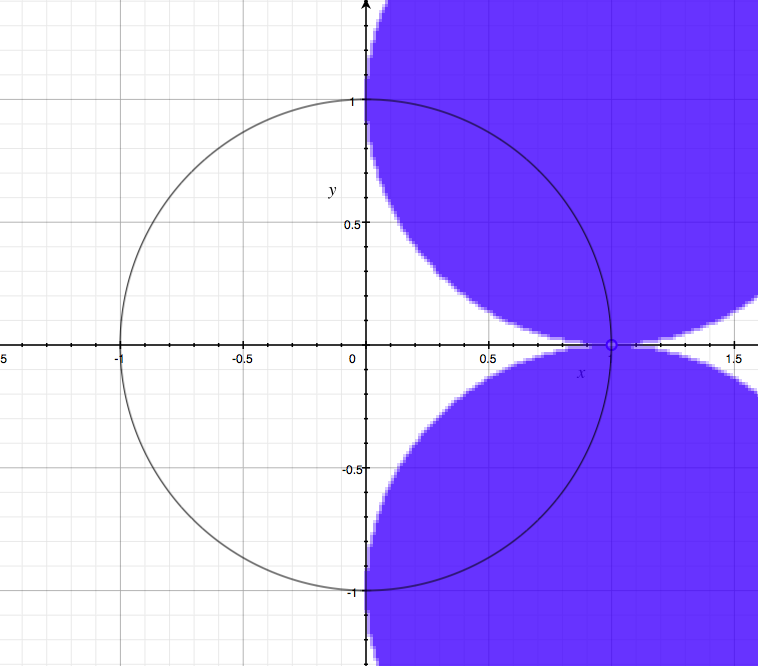
\includegraphics[scale=0.2]{hw7P526}
\end{center}
(b) Indeed $x^\ast = (1,0)$ satisfies the constraints. The gradient of Lagrangian is 
\begin{align*}
\nabla_x L(x^\ast, \lambda_1,\lambda_2) &= \nabla_x\l(\|x^\ast\|_2^2 + \lambda_1\l(\l\|x^\ast-\l[{1\atop 1}\r]\r\|^2 - 1\r) + \lambda_2\l(\l\|x^\ast-\l[{1\atop -1}\r]\r\|^2 - 1\r)\r) \\
&= 2x^\ast + 2\lambda_1\l(x^\ast-\l[{1\atop 1}\r]\r) + 2\lambda_2\l(x^\ast - \l[{1\atop -1}\r]\r) \\
&= \l[{2  \atop -2\lambda_1 + 2\lambda_2 }\r]
\end{align*}
Notice that there exists no $\lambda_1^\ast, \lambda_2^\ast$ that $\nabla_x L(x^\ast, \lambda_1^\ast,\lambda_2^\ast) = 0$ since the first entry of it is constantly 2. \\
\\
(c) From the above computation, we know the Lagrange dual function is not much but imposing $2x+ 2\lambda_1\l(x-\l[{1\atop 1}\r]\r) + 2\lambda_2\l(x - \l[{1\atop -1}\r]\r) = 0$ in the Lagrangian; this gives us
\begin{align*}
\bar x & = \/1{1+\lambda_1+\lambda_2}\l[{\lambda_1+\lambda_2 \atop \lambda_1 - \lambda_2}\r] \\
g(\lambda_1, \lambda_2) &= L(\bar x, \lambda_1, \lambda_2) \\
&= \frac{-(\lambda_1-\lambda_2)^2+\lambda_1+\lambda_2}{1+\lambda_1+\lambda_2}
\end{align*}
(may glory be to the great Wolfram Alpha) with the assumption that 
$1+\lambda_1+\lambda_2 > 0$ (we impose this to ensure Hessian of Lagrangian is positive definite to get infimum). The dual problem is 
\begin{align*}
\mbox{maximize\;\;\;} & \frac{-(\lambda_1-\lambda_2)^2+\lambda_1+\lambda_2}{1+\lambda_1+\lambda_2}\\
\mbox{subject to\;\;}& \lambda_1, \lambda_2 \geq 0
\end{align*}
with an implicit constraint $1+\lambda_1+\lambda_2 > 0$. Looking at the negative squared term we notice $\lambda_1 = \lambda_2$ needs to hold when maximized. The problem becomes maximizing $\/{t}{1+t}$ where $t = \lambda_1+\lambda_2 \geq 0$. This is bounded above by $1$ yet can't be maximized. Strong duality does not hold for this problem. (Notice that we failed Slater's condition for this one. ) \qed




\newpage\subsubsection*{Exercise 5.29 [Boyd \& Vandenberghe, 2004]}
{\it Ans:} Let $A = \l[\begin{array}{ccc}
-3 &&\\
&1&\\
&&2\end{array}\r]$; then take the Lagrangian and its gradient w.r.t. $x$,
\begin{align*}
L(x, \nu) &= x^T A x + 2\mathbf1^T x + \nu(\|x\|^2 - 1) \\
\nabla_xL(x,\nu) &= 2Ax + 2\mathbf1  + 2\nu x
\end{align*}
KKT condition suggests that $\nabla_xL(x^\ast, \nu^\ast) = 0$, \ie
$$x = (A+\nu I)^{-1} \mathbf 1 = \l[\begin{array}{c}
\frac1{\nu-3}\\
\frac1{\nu+1}\\
\frac1{\nu+2}
\end{array}\r]$$
and $\|x^\ast\|^2 = 1$, \ie
$$\l(\frac1{\nu-3}\r)^2 + \l(\frac1{\nu+1}\r)^2+\l(\frac1{\nu+2}\r)^2 = 1$$
Again, may glory be to the great Wolfram Alpha, this is equivalent to solving the sextic\footnote{OSX autocorrection does not recognize this word. It describes a polynomial to have degree 6. } polynomial equation $\nu^6 - 17 \nu^4 - 12 \nu^3 + 49 \nu^2 + 48 \nu -13 = 0$ which has 4 real roots $\nu^\ast \approx -3.14929, 0.223509, 1.8919, 4.03523$. Plug them into our objective function \begin{verbatim}
>> nu = [-3.14929, 0.223509, 1.8919, 4.03523];
>> x = @(nu) [1/(nu-3);1/(nu+1);1/(nu+2)];
>> A = diag([-3,1,2]);
>> obj = @(nu) x(nu)'*A*x(nu) + 2*sum(x(nu));
>> for  i=1:4
result(i) = obj(nu(i));
end
>> result

result =

   -1.3447    2.4972   -2.7910   -0.0444

\end{verbatim}
The optimum is $p^\ast \approx -2.7910$ which corresponds to $\nu^\ast \approx 1.8919$. \qed




\newpage\subsubsection*{Exercise 5.30 [Boyd \& Vandenberghe, 2004]}
{\it Ans:} Take the Lagrangian and its gradient w.r.t. $X$,
\begin{align*}
L(X, \nu) &= tr(X) - \log\det X + \nu^T (Xs - y)\\
\nabla_XL(X,\nu) &= diag(X) - \/1{\det X} adj(X) + \nu s^T \\
&= diag(X) - X^{-1} + \nu s^T
\end{align*}
To examine if $X^\ast = I + yy^T - \/1{\|s\|^2}ss^T$ is the optimal solution, first observe that $X^\ast s = s + y - s = y$, the equality constraint is satisfied. We use the Sherman-Morrison formula
$$(A+uv^T)^{-1} = A^{-1} - \frac{A^{-1}uv^TA^{-1}}{1+v^TA^{-1}u}$$
to help compute $(X^\ast)^{-1}$:
\begin{align*}
(I+yy^T)^{-1} &= I - \frac{yy^T}{1+\|y\|^2} \\
\l(I + yy^T - \/1{\|s\|^2}ss^T\r)^{-1} &= (I+yy^T)^{-1} + \frac{(I+yy^T)^{-1}ss^T(I+yy^T)^{-1}}{\|s\|^2-s^T(I+yy^T)^{-1}s} \\
&= I - \frac{yy^T}{1+\|y\|^2} + \frac{(I - \frac{yy^T}{1+\|y\|^2})ss^T(I - \frac{yy^T}{1+\|y\|^2})}{\|s\|^2-s^T(I - \frac{yy^T}{1+\|y\|^2})s}  \\
&= I - \frac{yy^T}{1+\|y\|^2} + \frac{(I - \frac{yy^T}{1+\|y\|^2})(ss^T - \frac{sy^T}{1+\|y\|^2})}{{1}/({1+\|y\|^2})}  \\
&= I - \frac{yy^T}{1+\|y\|^2} + \frac{ss^T - \frac{ys^T}{1+\|y\|^2} - \frac{sy^T}{1+\|y\|^2} + \frac{yy^T}{(1+\|y\|^2)^2}}
{{1}/({1+\|y\|^2})}  \\
&= I - \frac{yy^T}{1+\|y\|^2} + (1+\|y\|^2)ss^T - ys^T- sy^T + \frac{yy^T}{1+\|y\|^2}\\
&= I+ (1+\|y\|^2)ss^T - ys^T- sy^T\\
&= I + ss^T - sy^T
\end{align*}
(I have a feeling that I took a huge detour... anyways I verified the formula and indeed $(I+ss^T - sy^T)X^\ast = I$) Hence the gradient of Lagrangian condition becomes
\begin{align*}
\nabla_X L(X^\ast, \nu) &= diag(X^\ast) - I - ss^T + sy^T + \nu s^T \\
&= diag(yy^T) - \/1{\|s\|^2}diag(ss^T) - ss^T + sy^T + \nu s^T = 0
\end{align*}
But inspecting the diagonal entries of this matrix equation, we found
$$y_i^2 - \/1{\|s\|^2}s_i^2 - s_i^2 + s_iy_i + \nu_is_i = 0$$
Temporarily let $\nu_i = \/1{s_i}\l(-y_i^2 + \/1{\|s\|^2}s_i^2 + s_i^2 - s_iy_i \r)$. By inspection we know this will satisfy that $\nabla_XL(X^\ast, \nu) = 0$, the KKT conditions are satisfied, and $X^\ast$ is a optimal solution. \qed




\newpage\subsubsection*{Additional Exercise 4.10 [Boyd \& Vandenberghe, 2017]}
{\it Ans:} (a) The Lagrange function 
\begin{align*}
L(x, \nu) &= \|Ax-b\|^2_2 + x^T diag(\nu) x - \mathbf1^T\nu\\
&= b^Tb + x^T(A^TA + diag(\nu))x - 2b^TAx - \mathbf1^T\nu
\end{align*}
will be unbounded below if $A^TA + diag(\nu) \nsucceq 0$; hence under the assumption that $A^TA + diag(\nu) \succeq 0$, we can take derivative w.r.t. $x$ in order to find $g(\nu)$. 
\begin{align*}
\nabla_xL(x, \nu) &= 2(A^TA + diag(\nu))x - 2A^Tb = 0\\
x &= (A^TA + diag(\nu))^{-1}A^Tb\\
g(\nu) &= b^Tb - \mathbf1^T\nu -  b^TA(A^TA+diag(\nu))^{-1}A^Tb
\end{align*}
The dual problem is therefore a SDP:
\begin{align*}
\mbox{maximize\;\;\;} & b^Tb - \mathbf1^T\nu -  b^TA(A^TA+diag(\nu))^{-1}A^Tb \\
\mbox{subject to\;\;} & A^TA + diag(\nu) \succeq 0
\end{align*}
(b) Since there's a SDP constraint, the dual variable $Z \in \vS^n$ and the Lagrangian is 
\begin{align*}
L(\nu, Z) &= -b^Tb + \mathbf1^T\nu +  b^TA(A^TA+diag(\nu))^{-1}A^Tb - Z : (A^TA + diag(\nu)) \\
\nabla_\nu L(\nu, Z) &= \mathbf1 + (A^TA + diag(\nu))^{-1}A^Tb - diag(Z)
\end{align*}
This is from the fact that $\delta (A^{-1}) = A^{-1}\delta A A^{-1}$, 
$$\pd{(A^TA+diag(\nu))^{-1}}{\nu_i} = (A^TA+diag(\nu))^{-1}E_{ii}(A^TA+diag(\nu))^{-1}$$
where $E_{ii}$ denotes the matrix with $1$ at its $(i,i)$-th entry and $0$ for the rest. The gradient of Lagrangian can be zero if 
\begin{align*}
A^Tb &= (A^TA+diag(\nu))(diag(Z) - \mathbf1) \\
\nu_i &= (A_{ji}b_j - A_{ji}A_{jk}Z_{kk} + A_{ji}A_{jk}) / (Z_{ii}-1)
\end{align*}
Of course index notation can't help us better the understanding...

\newpage\subsubsection*{Additional Exercise 4.14 [Boyd \& Vandenberghe, 2017]}
{\it Ans:} (a) We verify that for $x = (1/2, 0, \cdots, 0, 1/2)$, indeed $x\succeq 0, \mathbf1^T x = 1$; due to complementary slackness, we impose $\lambda_1 = \lambda_n = 0$. The gradient of Lagrangian is then 
\begin{align*}
\nabla_x L(x, \lambda, \nu) &= \nabla_x \l(-\log(a^Tx) - \log(b^Tx) - \lambda^T x + \nu(\mathbf1^Tx-1)\r) \\
&= -\frac1{a^Tx}a - \frac1{b^Tx}b - \lambda + \nu\mathbf1 \\
&= \l[\begin{array}{c}
\nu - \/{2a_1}{a_1+a_n} - \/{2b_1}{b_1+b_n} \\
-\lambda_2 + \nu - \/{2a_2}{a_1+a_n} - \/{2b_2}{b_1+b_n} \\
\vdots\\
-\lambda_{n-1} + \nu - \/{2a_{n-1}}{a_1+a_n} - \/{2b_{n-1}}{b_1+b_n} \\
\nu - \/{2a_n}{a_1+a_n} - \/{2b_n}{b_1+b_n} \\
\end{array}\r]
\end{align*}
This can be solved since 
\begin{align*}
\frac{2a_1}{a_1+a_n} + \frac{2b_1}{b_1+b_n} &= \/{2a_1}{a_1+a_n} + \/{2\cdot \/1{a_1}}{\/1{a_1} + \/1{a_n}}\\
& = \/{2a_1}{a_1+a_n} + \/{2a_n}{a_1+a_n} = 2 \\
& = \/{2a_n}{a_1+a_n} + \/{2b_n}{b_1+b_n}
\end{align*}
we can let $\nu = 2$ then the first and $n$-th entries of the above gradient cancel.  Let $\lambda_i$ for $i=2, \cdots, n-1$ accordingly to cancel the terms, then
\begin{align*}
\lambda_i & = \nu - \/{2a_i}{a_1+a_n} - \/{2b_i}{b_1+b_n} \\
&= 2- \/{2a_i}{a_1+a_n} - \/{2b_i}{b_1+b_n} \geq 0
\end{align*}
(since $a_i$'s and $b_i$'s are in descending/ascending order) and the condition $\lambda \succeq 0$ is satisfied. \\
\\
(b) Consider the eigendecomposition $A = Q\Lambda Q^T$ and let $y = Q^Tu$, $x = y:y$ (\ie $x_i = y_i^2$ for $i=1, \cdots, n$), then the LHS of the inequality becomes
$$2\l(u^TAu\r)^{1/2}\l(u^TA^{-1}u\r)^{1/2} = 2\l(y^T\Lambda y\r)^{1/2}\l(y^T\Lambda^{-1}y\r)^{1/2} = 2(a^Tx)^{1/2}(b^Tx)^{1/2}$$
Due to part (a), we know the negative logarithm of this expression is bounded from below by substituting in $x^\ast = (1/2, 0, \cdots, 0, 1/2)$. Since negative logarithm is known to reverse order, we know now 
\begin{align*}
2\l(u^TAu\r)^{1/2}\l(u^TA^{-1}u\r)^{1/2} &= 2(a^Tx)^{1/2}(b^Tx)^{1/2}\\
&\leq 2(a^T x^\ast)^{1/2}(b^Tx^\ast)^{1/2} \\
&= 2\l(\frac{a_1+a_n}2\r)^{1/2}\l(\frac{b_1+b_n}2\r)^{1/2} \\
&= 2\l(\frac{\lambda_1+\lambda_n}2\r)^{1/2}\l(\frac{\lambda_n+\lambda_n}{2\lambda_1\lambda_n}\r)^{1/2} \\
&= \frac{\lambda_1+\lambda_n}{\lambda_1^{1/2}\lambda_n^{1/2}} \\
&= \sqrt{\frac{\lambda_1}{\lambda_n}} + \sqrt{\frac{\lambda_n}{\lambda_1}}
\end{align*}
\qed





\newpage\subsubsection*{Additional Exercise 4.17 [Boyd \& Vandenberghe, 2017]}
{\it Ans:} (a) \\
\underline{``$tr(AX^\ast) \geq f(A)$": } Take the unit eigenvectors $v_1, \cdots, v_r$ corresponding to $\lambda_1(A), \cdots, \lambda_r(A)$ and let 
$X = \SUM{i=1}r v_iv_i^T$, then 
$$tr(AX) = \SUM{i=1}r tr(Av_iv_i^T) = \SUM{i=1}r tr(v_i^TAv_i) = \SUM{i=1}r \lambda_i(A)$$
Now enough to show that $X$ satisfies the constraints of the problem. First we observe 
$$tr(X) = \SUM{i=1}r tr(v_iv_i^T) = \SUM{i=1}r tr(v_i^Tv_i) = \SUM{i=1}r \|v_i\|^2_2 = r$$
Secondly, $X$ is certainly semi-positive definite (it's the sum of $r$ semi-positive definite matrices), and for any $x \in \R^n$, 
$$x^T (I - X) x = \SUM{i=1}r \|x\|^2 - (x^T v_i)^2 \geq 0$$
due to Cauchy's inequality, and $X \preceq I$. \\
\\
\underline{``$tr(AX^\ast) \leq f(A)$": } Suppose $X \in \vS^n$ satisfies the constraints $tr(X) = r, 0 \preceq X \preceq I$; take the eigendecomposition $X = UM U^T$ with the diagonals of $M$ being $\mu_1 \geq \mu_2 \geq \cdots \geq \mu_n$, then from the constraints we know $\SUM{i=1}n \mu_i = r$ and $0 \leq \mu_i \leq 1$ for all $i=1, \cdots, n$. Now from the cyclic property of trace, 
\begin{align*}
tr(AX) &= tr(AUM U^T) \\
&= tr(U^T AU M) \\
&= diag(U^TAU) : M \\
&= \SUM{i=1}n \mu_i u_i^T A u_i
\end{align*}
(Here $A:B = \SUM{i,j = 1}n a_{ij}b_{ij}$ denotes the entry-wise product. ) From the ordering that $1\geq \mu_1\geq \mu_2 \geq \cdots \geq \mu_n \geq 0$ we notices this is bounded by $\SUM{i=1}n \mu_i \lambda_i(A)$ due to min-max principle and that $u_i$'s form a basis. Along with the constraint that $\SUM{i=1}n \mu_i = r$ we can see now 
$$\tr(AX) = \SUM{i=1}n \mu_i u_i^T A u_i \leq \SUM{i=1}n \mu_i \lambda_i(A) \leq \SUM{i=1}r \lambda_i(A) = f(A)$$
(b) Utilize the result from part (a); denote the feasible set of problem in (a) by 
$$S = \{X \in \vS^n \mid tr(X) = r,0\preceq X \preceq I\}$$. Take $\theta \in [0,1]$ and $A, B \in \vS^n$, then 
\begin{align*}
f(\theta A + (1-\theta)B) &= \max_{X \in S} tr((\theta A + (1-\theta)B)X)\\
&= \max_{X \in S} \theta tr(AX) + (1-\theta) tr(BX) \\
&\leq \theta \max_{X\in S} tr(AX) + (1-\theta) \max_{Y \in S} tr(BY) \\
&= \theta f(A) + (1-\theta)f(B)
\end{align*} 
(c) With the above derivations, we now know the problem is equivalent to
\begin{align*}
\mbox{minimize\;\;\;} & t\\
\mbox{subject to\;\;} & y_0 + x^Ty \leq t \\
& y_i = tr(A_i X), \mbox{ for }i = 0, 1, \cdots, m\\
& tr(X) = r \\
& 0 \preceq X \preceq I
\end{align*}
Note here the variable $y = \l[\begin{array}{c}
y_1\\
\vdots\\
y_m\end{array}\r]$ excludes the digit $y_0$. \qed




\newpage\subsubsection*{Additional Exercise 4.18 [Boyd \& Vandenberghe, 2017]}
I accidentally did this problem...\\
{\it Ans:} (a) The maximum of several convex functions is convex, and taking linear combination of two convex functions with positive coefficients is still convex. \\
\\
(b) Denote the Lagrange dual function for problem (16) by
$$g_{16}(\lambda) = \inf_x f_0(x) + \SUM{i=1}m \lambda_if_i(x)$$
where $\lambda = [\lambda_1, \cdots, \lambda_m]^T$; then the Lagrangian and the Lagrange dual function for problem (19) is (with one more dual variable $\lambda_0$ due to the constraint $y\leq 0$)
\begin{align*}
L_{19}(x, y, \lambda_0, \lambda) & = f_0(x) + ty + \SUM{i=1}m \lambda_i(f_i(x) - y) + \lambda_0 y \\
& = f_0(x) + \SUM{i=1}m \lambda_i f_i(x) + \l(t + \lambda_0 - \SUM{i=1}m \lambda_i\r)y \\
g_{19}(\lambda_0, \lambda) & = \inf_{x, y} L(x, y, \lambda) \\
&= g_{16}(\lambda) + \inf_y \l(t + \lambda_0 - \SUM{i=1}m \lambda_i\r)y \\
&= \casebrak{g_{16}(\lambda)}{t + \lambda_0 - \SUM{i=1}m \lambda_i = 0}{-\infty}{\mbox{else}}
\end{align*}
(c) Assume $t > \mathbf1^T\lambda^\ast$, then $g_{19}(\mathbf1^T\lambda^\ast - t, \lambda)$ can attain its maximum $g_{16}(\lambda^\ast)$. Under the assumption of Slater's condition, optimal solution $(x^\ast, y^\ast)$ to problem (19) (which is equivalent to problem (18) if we take only $x^\ast$) will give the same optimal value $g_{19}(\lambda^\ast)$ as problem (16). Since problem (18) is ``weaker" than problem (16) (\ie optimal solution to problem (16) will also solve problem (18)), we know then $x^\ast$ solves problem (16). \qed


\end{document}
